% @Author: Takwa Ben Aïcha Gader
% @Date:   2026-02-20
% @Last Modified time: 2026-05-30

%%%%%%%%%%%%%%%%%%%%%%%%%%%%
% CHAPITRE 4               %
%%%%%%%%%%%%%%%%%%%%%%%%%%%%
\chapter{Réalisation — Espace Étudiant}
\label{chap:realisation_etudiant}

%%%%%%%%%%%%%%%%%%%%%%%%%%%%%%%%%%%%%%%%%%%%%%%%%%%%
\section*{Introduction}
\addcontentsline{toc}{section}{Introduction}

Après avoir exposé la modélisation conceptuelle et détaillé les fondements théoriques des algorithmes décisionnels de la plateforme \textbf{CapAvenir}, ce chapitre présente la réalisation concrète et l'implémentation physique de l'Espace Étudiant. Constituant le cœur applicatif du système, cet espace gère l'interaction directe et séquentielle de l'apprenant avec les services d'aide à la décision. 

Afin de garantir une appropriation optimale de la plateforme par des bacheliers en phase de transition académique, l'Espace Étudiant a été conçu selon trois principes directeurs d'ergonomie et d'ingénierie cognitive, schématisés par la figure~\ref{fig:principes_espace_etudiant}.

\begin{figure}[H]
\centering
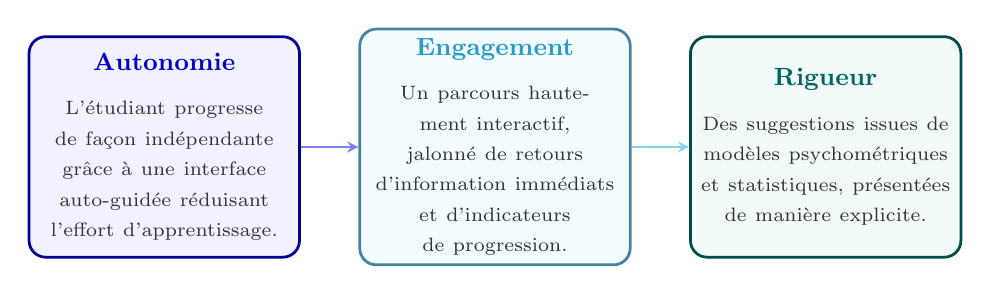
\begin{tikzpicture}[
  every node/.style={align=center, font=\small},
  pblue/.style={draw=blue!60!black, fill=blue!5, rounded corners=6pt,
                minimum width=3.4cm, minimum height=2.8cm, text width=3.2cm, line width=1pt},
  pmidblue/.style={draw=cyan!60!black, fill=cyan!5, rounded corners=6pt,
                minimum width=3.4cm, minimum height=2.8cm, text width=3.2cm, line width=1pt},
  pdarkblue/.style={draw=teal!60!black, fill=teal!5, rounded corners=6pt,
                  minimum width=3.4cm, minimum height=2.8cm, text width=3.2cm, line width=1pt}
]
\node[pblue] (n1) at (0,0) {
  {\color{blue!80!black}\textbf{Autonomie}}\\[5pt]
  {\color{black!80}\scriptsize L'étudiant progresse de façon indépendante grâce à une interface auto-guidée réduisant l'effort d'apprentissage.}
};
\node[pmidblue] (n2) at (4.2,0) {
  {\color{cyan!80!black}\textbf{Engagement}}\\[5pt]
  {\color{black!80}\scriptsize Un parcours hautement interactif, jalonné de retours d'information immédiats et d'indicateurs de progression.}
};
\node[pdarkblue] (n3) at (8.4,0) {
  {\color{teal!80!black}\textbf{Rigueur}}\\[5pt]
  {\color{black!80}\scriptsize Des suggestions issues de modèles psychométriques et statistiques, présentées de manière explicite.}
};
\draw[->, thick, blue!50, >=stealth] (n1.east) -- (n2.west);
\draw[->, thick, cyan!50, >=stealth] (n2.east) -- (n3.west);
\end{tikzpicture}
\caption{Les trois principes directeurs de l'Espace Étudiant}
\label{fig:principes_espace_etudiant}
\end{figure}

Dans les sections suivantes, nous détaillons les aspects techniques et ergonomiques des différentes interfaces jalonnant ce module, depuis l'accès hautement sécurisé par authentification forte jusqu'à l'exploration des recommandations et la génération automatisée d'outils de candidature.

%%%%%%%%%%%%%%%%%%%%%%%%%%%%%%%%%%%%%%%%%%%%%%%%%%%%
\section{Le parcours de l'étudiant : vue d'ensemble}
\label{sec:parcours_etudiant}

Le parcours de l'étudiant au sein de la plateforme suit un enchaînement logique et progressif structuré en huit modules clés. Cet enchaînement a été modélisé de façon à accompagner l'étudiant de la collecte d'informations initiales jusqu'à la modélisation de scénarios futurs et de supports de candidature. La figure~\ref{fig:parcours_global} schématise l'ordre séquentiel de ces étapes au sein de l'application.

\begin{figure}[H]
\centering
\begin{tikzpicture}[
    node distance=0.5cm,
    block/.style={rectangle, draw=blue!70!black, fill=blue!5, rounded corners=3pt, minimum width=6.2cm, minimum height=0.75cm, align=center, font=\small},
    arrow/.style={-latex, thick, draw=blue!60!black}
]
    \node[block] (auth) {1. Authentification Double Facteur (2FA)};
    \node[block, below=of auth] (profil) {2. Saisie du profil académique};
    \node[block, below=of profil] (calc) {3. Calculateur de Formule Globale (FG)};
    \node[block, below=of calc] (test) {4. Évaluation psychométrique adaptative};
    \node[block, below=of test] (reco) {5. Recommandations personnalisées (SIAEPI)};
    \node[block, below=of reco] (catalogue) {6. Catalogue général des formations};
    \node[block, below=of catalogue] (simu) {7. Simulateur décisionnel What-If \& Comparateur};
    \node[block, below=of simu] (cv) {8. Générateur de Curriculum Vitae (CV Builder)};

    \draw[arrow] (auth) -- (profil);
    \draw[arrow] (profil) -- (calc);
    \draw[arrow] (calc) -- (test);
    \draw[arrow] (test) -- (reco);
    \draw[arrow] (reco) -- (catalogue);
    \draw[arrow] (catalogue) -- (simu);
    \draw[arrow] (simu) -- (cv);
\end{tikzpicture}
\caption{Parcours séquentiel de l'étudiant dans la plateforme CapAvenir}
\label{fig:parcours_global}
\end{figure}

Chacune de ces étapes fait l'objet d'une analyse d'implémentation fonctionnelle et technique dans la suite de ce chapitre.

%%%%%%%%%%%%%%%%%%%%%%%%%%%%%%%%%%%%%%%%%%%%%%%%%%%%
\section{Authentification et double facteur (2FA)}
\label{sec:auth_etudiant}

\subsection{Fonctionnalité et Sécurisation}

L'accès à l'Espace Étudiant implique la manipulation de données personnelles et académiques sensibles (notes scolaires, profils psychologiques, coordonnées). Afin de se prémunir contre les risques d'usurpation d'identité et de sécuriser l'accès aux données, la plateforme implémente un protocole d'authentification forte à double facteur (2FA). 

Après la vérification standard des identifiants (adresse email et mot de passe chiffré via l'algorithme robuste \texttt{bcrypt}), le système génère un jeton OTP (\textit{One-Time Password}) numérique à six chiffres. Ce jeton, lié à la session de l'utilisateur, possède une durée de validité limitée à dix minutes. Il est transmis instantanément à l'étudiant par courriel via une passerelle de messagerie sécurisée. L'accès définitif à la plateforme n'est autorisé qu'après validation du code reçu.

\subsection{Interfaces Utilisateur}

L'interface a été conçue pour offrir un parcours fluide et sans friction visuelle, en exploitant les composants dynamiques de Tailwind CSS. La figure~\ref{fig:auth_etudiant} présente la mire de connexion initiale ainsi que l'interface dédiée à la saisie du code de sécurité OTP.

\begin{figure}[H]
    \centering
    \begin{subfigure}[b]{0.48\textwidth}
        \centering
        \includegraphics[width=\textwidth]{images/auth_login.png}
        \caption{Mire d'authentification initiale}
        \label{fig:auth_login}
    \end{subfigure}
    \hfill
    \begin{subfigure}[b]{0.48\textwidth}
        \centering
        \includegraphics[width=\textwidth]{images/auth_verification.png}
        \caption{Saisie du jeton OTP temporaire}
        \label{fig:auth_verification}
    \end{subfigure}
    \caption{Processus d'authentification sécurisée à double facteur (2FA)}
    \label{fig:auth_etudiant}
\end{figure}

%%%%%%%%%%%%%%%%%%%%%%%%%%%%%%%%%%%%%%%%%%%%%%%%%%%%
\section{Tableau de bord personnalisé}
\label{sec:dashboard_etudiant}

\subsection{Fonctionnalité et Ergonomie}

Le tableau de bord constitue l'écran d'accueil et le cockpit de pilotage de l'étudiant après son authentification. Son objectif principal est de synthétiser en une seule vue logique l'état d'avancement du bachelier dans son parcours d'orientation et de lui offrir un accès rapide aux différents modules décisionnels. Il est bâti sur une architecture de composants asynchrones permettant la mise à jour des widgets sans rechargement global de la page.

\subsection{Composants Applicatifs Principaux}

\begin{itemize}
    \item \textbf{Widget de Progression} : Il affiche un indicateur circulaire interactif traduisant le taux d'achèvement des étapes obligatoires du parcours d'orientation (validation des notes, passation du test d'orientation, consultation des recommandations).
    \item \textbf{Radar de Compétences et Code Holland} : Ce composant intègre un graphique vectoriel interactif (radar) généré dynamiquement à partir des scores normalisés obtenus lors de l'évaluation psychométrique. Il expose le profil de Holland dominant sous forme de code à trois lettres (ex. \textit{RIA}).
    \item \textbf{Espace d'Actions Directes} : Une grille de raccourcis ergonomiques structurés permet à l'utilisateur d'initier le pipeline d'orientation, d'interagir avec l'assistant virtuel Nova, de concevoir un CV ou de simuler des notes.
\end{itemize}

\begin{figure}[H]
    \centering
    \includegraphics[width=0.85\textwidth]{images/tableau_de_bord_etudiant.png}
    \caption{Tableau de bord personnalisé de l'étudiant}
    \label{fig:dashboard_etudiant_view}
\end{figure}

%%%%%%%%%%%%%%%%%%%%%%%%%%%%%%%%%%%%%%%%%%%%%%%%%%%%
\section{Profil académique et saisie des notes}
\label{sec:profil_academique}

\subsection{Fonctionnalité et Validation Dynamique}

Cette interface permet à l'étudiant de renseigner sa section du baccalauréat tunisien et de saisir les notes associées à chaque matière pour la session principale. La spécificité technique de ce module repose sur l'adaptation dynamique du formulaire : dès que l'étudiant sélectionne sa section (ex. \textit{Informatique} ou \textit{Technique}), le système charge en mémoire les coefficients et les matières requis à l'aide de liaisons de données bidirectionnelles (système de réactivité réactif).

Afin d'assurer l'intégrité des calculs ultérieurs, des validations strictes sont appliquées côté client et côté serveur, garantissant que chaque note saisie appartient à l'intervalle réel $[0, 20]$ et bloquant toute soumission de données incohérentes.

\subsection{Interface Utilisateur}

La figure~\ref{fig:profil_academique_interface} illustre l'adaptation dynamique de l'interface, depuis le formulaire vierge initial demandant le choix de la section jusqu'à la saisie des notes pour les matières correspondantes.

\begin{figure}[H]
    \centering
    \begin{subfigure}[b]{0.48\textwidth}
        \centering
        \includegraphics[width=\textwidth]{images/profil_academique_vide.png}
        \caption{Sélection de la section d'origine}
        \label{fig:profil_academique_vide}
    \end{subfigure}
    \hfill
    \begin{subfigure}[b]{0.48\textwidth}
        \centering
        \includegraphics[width=\textwidth]{images/profil_academique_rempli.png}
        \caption{Champs de saisie des notes par matière}
        \label{fig:profil_academique_rempli}
    \end{subfigure}
    \caption{Interface de configuration du profil académique}
    \label{fig:profil_academique_interface}
\end{figure}

%%%%%%%%%%%%%%%%%%%%%%%%%%%%%%%%%%%%%%%%%%%%%%%%%%%%
\section{Pipeline d'orientation unifié}
\label{sec:pipeline_orientation}

Le pipeline d'orientation unifié est un composant qui formalise le parcours obligatoire de l'utilisateur sous la forme d'un assistant linéaire (\textit{wizard}). Ce choix de conception vise à réduire la charge mentale de l'étudiant en hiérarchisant les étapes critiques. L'accès aux étapes est contrôlé par une machine à états finis intégrée au backend Laravel :
\begin{enumerate}
    \item \textbf{Étape 1 : Profil académique} (Saisie ou modification des notes de baccalauréat).
    \item \textbf{Étape 2 : Évaluation adaptative} (Passation du test ou consultation directe des scores si déjà complété).
    \item \textbf{Étape 3 : Recommandations personnalisées} (Génération des listes de filières optimales).
\end{enumerate}

Le pipeline gère les verrous de sécurité applicatifs : l'étudiant ne peut accéder aux étapes ultérieures sans avoir complété et validé les précédentes.

\subsection{Interface Utilisateur}

Cette interface fournit un suivi visuel en temps réel de la progression de l'étudiant tout au long du processus d'orientation. Chaque étape franchie est marquée d'un indicateur de complétion, et les étapes suivantes sont dynamiquement déverrouillées au fur et à mesure de l'avancement.

\vspace{0.8cm}
\begin{figure}[H]
    \centering
    \fbox{\parbox{0.85\textwidth}{\centering \vspace{1.5cm} Capture d'écran : Interface du pipeline d'orientation unifié avec progression visuelle et étapes dynamiques \vspace{1.5cm}}}
    \caption{Interface du pipeline d'orientation unifié}
    \label{fig:pipeline_orientation_screen}
\end{figure}

%%%%%%%%%%%%%%%%%%%%%%%%%%%%%%%%%%%%%%%%%%%%%%%%%%%%
\section{Test d'évaluation du profil}
\label{sec:test_cat}

\subsection{Fonctionnalité et Modélisation Adaptative (CAT)}

Cette interface pilote la passation du test d'orientation. Contrairement aux évaluations psychométriques classiques et statiques, la plateforme intègre un moteur de test adaptatif informatisé (\textit{Computerized Adaptive Testing} - CAT) s'appuyant sur la Théorie de Réponse aux Items (IRT). Plus précisément, le système modélise l'interaction étudiant-item via la fonction logistique à deux paramètres (modèle IRT 2PL). Pour chaque item $i$, la probabilité qu'un étudiant ayant un trait latent $\theta$ donne une réponse affirmative est modélisée par la formule~\ref{eq:irt_2pl_realisation}.

\begin{equation}
P(X_i = 1 \mid \theta) = \frac{1}{1 + e^{-D a_i(\theta - b_i)}}
\label{eq:irt_2pl_realisation}
\end{equation}

Où :
\begin{itemize}
    \item $\theta$ représente le niveau d'intérêt latent de l'étudiant dans une dimension spécifique (borné théoriquement entre $-3$ et $+3$).
    \item $a_i$ désigne le paramètre de discrimination de l'item $i$ (sensibilité de la question aux variations du trait latent).
    \item $b_i$ représente le paramètre de difficulté de l'item $i$ (niveau de trait nécessaire pour valider l'item).
    \item $D$ est un facteur d'échelle constant égal à $1{,}702$.
\end{itemize}

Le test est divisé en trois phases complémentaires :
\begin{enumerate}
    \item \textbf{Phase 1 : Couverture obligatoire (Questions 1 à 30)} : garantit que chacune des six dimensions de Holland obtient au moins 3 réponses.
    \item \textbf{Phase 2 : Intercalage cognitif} : injecte de manière séquentielle toutes les 6 questions un item d'évaluation GATB pour mesurer les aptitudes logiques et spatiales.
    \item \textbf{Phase 3 : Sélection adaptative fine (Q30+)} : choisit dynamiquement à chaque étape l'item maximisant l'information de Fisher relative au trait estimé de l'étudiant.
\end{enumerate}

Le test s'interrompt automatiquement (\textit{early stopping}) lorsque l'erreur-type de mesure (SEM) descend sous un seuil critique de $0{,}15$ ou après un maximum de 50 questions, évitant ainsi la fatigue cognitive de l'étudiant. De plus, un module d'analyse comportementale évalue le temps de réponse pour chaque question (alertant en cas de clic trop rapide inférieur à 500 ms) afin de garantir la sincérité des données récoltées.

\subsection{Interface Utilisateur}

\begin{figure}[H]
    \centering
    \begin{subfigure}[b]{0.48\textwidth}
        \centering
        \includegraphics[width=\textwidth]{images/test_intro.png}
        \caption{Écran d'introduction et consignes}
        \label{fig:test_intro}
    \end{subfigure}
    \hfill
    \begin{subfigure}[b]{0.48\textwidth}
        \centering
        \includegraphics[width=\textwidth]{images/test_question.png}
        \caption{Passation d'un item avec échelle de Likert}
        \label{fig:test_question}
    \end{subfigure}
    \caption{Interface adaptative de passation du test d'orientation}
    \label{fig:test_cat_interface}
\end{figure}

%%%%%%%%%%%%%%%%%%%%%%%%%%%%%%%%%%%%%%%%%%%%%%%%%%%%
\section{Résultats du test et profil d'orientation}
\label{sec:resultats_riasec}

\subsection{Fonctionnalité et Restitution Statistique}

Dès la clôture de l'évaluation adaptative, le système calcule et normalise les scores de l'étudiant sur une échelle de $0$ à $100$ pour chacune des six dimensions du modèle de Holland. Les calculs intègrent un indice de cohérence interne (coefficient Alpha de Cronbach, formule~\ref{eq:cronbach}) pour s'assurer de la stabilité des réponses. Si ce coefficient est inférieur à $0{,}60$, le profil est marqué pour révision.

\begin{equation}
\alpha = \frac{k}{k - 1} \left( 1 - \frac{\sum_{i=1}^k \sigma^2_{Y_i}}{\sigma^2_X} \right)
\label{eq:cronbach}
\end{equation}

Où $k$ représente le nombre d'items du test, $\sigma^2_{Y_i}$ la variance de l'item $i$, et $\sigma^2_X$ la variance totale du score obtenu. Le code Holland final (constitué des trois dimensions dominantes triées par ordre décroissant) est ensuite généré.

\subsection{Interface de Visualisation}

L'interface de restitution graphique intègre un composant vectoriel interactif SVG représentant le radar psychométrique de Holland. La figure~\ref{fig:resultats_riasec_screen} présente l'interface d'affichage de ces résultats.

\begin{figure}[H]
    \centering
    \includegraphics[width=0.85\textwidth]{images/resultats_riasec.png}
    \caption{Interface de restitution des résultats du test et profil psychométrique}
    \label{fig:resultats_riasec_screen}
\end{figure}

Le tableau~\ref{tab:riasec_dim} résume la taxonomie des six dimensions théoriques utilisées pour classifier les intérêts de l'étudiant.

\begin{table}[H]
\centering
\renewcommand{\arraystretch}{1.3}
\begin{tabular}{|>{\columncolor{blue!5}}c|p{3.2cm}|p{8.8cm}|}
\hline
\rowcolor{blue!15}
\textbf{Code} & \textbf{Profil Vocationnel} & \textbf{Caractéristiques et Préférences Professionnelles} \\
\hline
\textbf{R} & Réaliste & Manipulation d'objets, machines, outils. Intérêt pour le concret et l'extérieur. \\ \hline
\textbf{I} & Investigateur & Activités de recherche, analyse de données, résolution de problèmes abstraits. Esprit scientifique. \\ \hline
\textbf{A} & Artistique & Création esthétique, expression personnelle littéraire ou visuelle. Indépendance et originalité. \\ \hline
\textbf{S} & Social & Aide, conseil, enseignement, soin à la personne et activités coopératives. \\ \hline
\textbf{E} & Entreprenant & Leadership, influence, prise de décision managériale, négociation et persuasion. \\ \hline
\textbf{C} & Conventionnel & Traitement structuré des données, ordre, classement, respect des consignes et rigueur administrative. \\ \hline
\end{tabular}
\caption{Les six dimensions fondamentales du modèle RIASEC}
\label{tab:riasec_dim}
\end{table}

%%%%%%%%%%%%%%%%%%%%%%%%%%%%%%%%%%%%%%%%%%%%%%%%%%%%
\section{Recommandations personnalisées}
\label{sec:recommandations_siaepi}

\subsection{Fonctionnalité et Appariement Algorithmique (SIAEPI)}

Cette interface restitue les filières d'études supérieures tunisiennes les plus adaptées au profil de l'étudiant. Les recommandations sont calculées par le moteur de recommandation hybride SIAEPI v8.0. Ce moteur applique une similarité cosinus (formule~\ref{eq:cosine}) pour évaluer la correspondance entre le vecteur psychométrique de l'étudiant ($V_e$) et le profil cible de chaque filière ($V_f$) stocké en base de données.

\begin{equation}
\text{Sim}(V_e, V_f) = \frac{V_e \cdot V_f}{\|V_e\| \cdot \|V_f\|} = \frac{\sum_{i=1}^6 v_{e,i} \cdot v_{f,i}}{\sqrt{\sum_{i=1}^6 v_{e,i}^2} \cdot \sqrt{\sum_{i=1}^6 v_{f,i}^2}}
\label{eq:cosine}
\end{equation}

Les résultats sont enrichis d'un système de classification en quatre onglets stratégiques, basé sur la comparaison entre le score FG de l'étudiant et le Score de Dernier Orienté historique (SDO) de la formation :
\begin{itemize}
    \item \textbf{Choix Ambitieux} : Formations compétitives dont le SDO est légèrement supérieur au score FG de l'étudiant, mais accessibles en cas de désistements.
    \item \textbf{Top Recommandations} : Cœur des filières optimales qui maximisent la compatibilité RIASEC et garantissent un niveau d'admissibilité très élevé.
    \item \textbf{Opportunités Accessibles} : Formations sécurisantes situées en dessous du score FG de l'étudiant, offrant de bons taux d'insertion.
    \item \textbf{Filières de repli} : Choix de sécurité garantissant une affectation universitaire en cas de forte pression sélective nationale.
\end{itemize}

\subsection{Fonctionnalités Interactives Avancées}

\begin{itemize}
    \item \textbf{Système de Rétroaction Dynamique (Feedback)} : L'étudiant peut attribuer une note (de 1 à 5 étoiles) ou indiquer une préférence binaire sur chaque suggestion. Ces interactions sont stockées en base de données pour affiner les prédictions ultérieures du moteur d'apprentissage.
    \item \textbf{Gap Analysis (Analyse des Écarts)} : Un module compare le score FG réel de l'étudiant par rapport au SDO historique des trois dernières sessions nationales d'orientation, lui indiquant explicitement sa viabilité d'admission.
    \item \textbf{Fiche Métiers (Career Accordion)} : Un volet dépliant intègre des données socio-économiques du marché tunisien de l'emploi (taux d'employabilité officiel, salaires médians par secteur d'activité, métiers associés).
\end{itemize}

\begin{figure}[H]
    \centering
    \includegraphics[width=0.85\textwidth]{images/recommandations.png}
    \caption{Interface de recommandation de formations structurées par niveau de sélectivité}
    \label{fig:recommandations_screen}
\end{figure}

%%%%%%%%%%%%%%%%%%%%%%%%%%%%%%%%%%%%%%%%%%%%%%%%%%%%
\section{Catalogue général des formations}
\label{sec:catalogue_orientation}

\subsection{Fonctionnalité et Filtres Multicritères}

Pour lever les contraintes de filtrage du moteur de recommandation, l'Espace Orientation propose un catalogue général répertoriant l'ensemble de l'offre académique tunisienne (plus de 2200 filières actives réparties sur les universités publiques). 

L'étudiant dispose d'un moteur de recherche textuel indexé ainsi que de filtres basés sur la taxonomie académique nationale (filtrage par domaine d'enseignement, par établissement d'attache ou par gouvernorat). Pour chaque formation consultée, le catalogue expose l'évolution des scores SDO sur les années 2023, 2024 et 2025. Cela permet à l'étudiant de mesurer la dynamique sélective de chaque filière et d'ajuster ses choix stratégiques.

\subsection{Interface Utilisateur}

\begin{figure}[H]
    \centering
    \includegraphics[width=0.85\textwidth]{images/espace_orientation.png}
    \caption{Interface d'exploration du catalogue général des formations}
    \label{fig:espace_orientation_screen}
\end{figure}

%%%%%%%%%%%%%%%%%%%%%%%%%%%%%%%%%%%%%%%%%%%%%%%%%%%%
\section{Simulateur décisionnel What-If}
\label{sec:simulateur_whatif}

\subsection{Fonctionnalité et Modélisation Multi-facettes}

Le simulateur décisionnel What-If offre aux étudiants la possibilité de projeter virtuellement des scénarios de notes académiques ou de choix de sections et d'en évaluer instantanément l'impact sur leur orientation. L'interface orchestre six sous-modules d'analyse intégrés au sein d'une même interface réactive :

\begin{enumerate}
    \item \textbf{Simulation par notes (Curseurs)} : Ajustement des notes des matières à l'aide de curseurs et recalcul en temps réel du score de Formule Globale (FG) et de la liste des formations débloquées.
    \item \textbf{Simulation de changement de spécialité} : Analyse comparative de l'impact sur le score FG si l'étudiant avait préparé une autre section de baccalauréat.
    \item \textbf{Comparateur de filières alternatives} : Visualisation sous forme de fiches des options d'orientation connexes en cas de score FG insuffisant pour le vœu principal.
    \item \textbf{Marché du travail et tendances} : Projection statistique de l'évolution de la demande du secteur professionnel ciblé à l'horizon des 5 prochaines années.
    \item \textbf{Retour sur investissement (ROI)} : Évaluation du coût théorique des études par rapport aux prévisions de salaires médians à l'embauche sur le marché tunisien et international.
    \item \textbf{Compatibilité de carrière (RIASEC)} : Calcul de la cohérence globale entre le profil psychométrique actuel de l'étudiant et les exigences opérationnelles du métier visé.
\end{enumerate}

Le système intègre un module d'historique persistant : l'étudiant peut sauvegarder ses différentes simulations académiques sous des étiquettes personnalisées afin de les comparer ultérieurement.

\subsection{Interface de Simulation}

\begin{figure}[H]
    \centering
    \begin{subfigure}[b]{0.48\textwidth}
        \centering
        \includegraphics[width=\textwidth]{images/simulateur_notes.png}
        \caption{Simulation selon les notes de l'étudiant}
        \label{fig:simulateur_notes}
    \end{subfigure}
    \hfill
    \begin{subfigure}[b]{0.48\textwidth}
        \centering
        \includegraphics[width=\textwidth]{images/simulateur_specialite.png}
        \caption{Simulation de changement de spécialité}
        \label{fig:simulateur_specialite}
    \end{subfigure}
    
    \vspace{0.3cm}
    
    \begin{subfigure}[b]{0.48\textwidth}
        \centering
        \includegraphics[width=\textwidth]{images/simulateur_filieres_alt.png}
        \caption{Comparateur de filières alternatives}
        \label{fig:simulateur_filieres_alt}
    \end{subfigure}
    \hfill
    \begin{subfigure}[b]{0.48\textwidth}
        \centering
        \includegraphics[width=\textwidth]{images/simulateur_employabilite.png}
        \caption{Marché du travail et employabilité}
        \label{fig:simulateur_employabilite}
    \end{subfigure}
    
    \vspace{0.3cm}
    
    \begin{subfigure}[b]{0.48\textwidth}
        \centering
        \includegraphics[width=\textwidth]{images/simulateur_roi.png}
        \caption{Retour sur investissement (ROI)}
        \label{fig:simulateur_roi}
    \end{subfigure}
    \hfill
    \begin{subfigure}[b]{0.48\textwidth}
        \centering
        \includegraphics[width=\textwidth]{images/simulateur_carriere.png}
        \caption{Compatibilité de carrière (RIASEC)}
        \label{fig:simulateur_carriere}
    \end{subfigure}
    \caption{Interface multi-facettes du simulateur What-If}
    \label{fig:simulateur_whatif}
\end{figure}

%%%%%%%%%%%%%%%%%%%%%%%%%%%%%%%%%%%%%%%%%%%%%%%%%%%%
\section{Comparateur de filières}
\label{sec:comparateur}

\subsection{Fonctionnalité et Alignement Critère par Critère}

Le module Comparateur permet à l'étudiant de sélectionner jusqu'à trois filières universitaires afin de les évaluer côte à côte sur une grille d'analyse standardisée. Les critères de comparaison intègrent des dimensions hétérogènes :
\begin{itemize}
    \item L'adéquation psychologique calculée (pourcentage de concordance RIASEC).
    \item La sélectivité d'accès (comparaison des scores SDO historiques par rapport au score FG de l'étudiant).
    \item L'employabilité sectorielle (temps moyen de recherche du premier emploi et salaire médian constaté).
    \item La contrainte géographique (localisation de l'établissement d'accueil).
\end{itemize}

L'étudiant peut exporter ou partager le rapport de comparaison généré au format de document léger.

\subsection{Interface Utilisateur}

\begin{figure}[H]
    \centering
    \includegraphics[width=0.85\textwidth]{images/comparateur.png}
    \caption{Interface d'évaluation comparative côte-à-côte des filières}
    \label{fig:comparateur_screen}
\end{figure}

%%%%%%%%%%%%%%%%%%%%%%%%%%%%%%%%%%%%%%%%%%%%%%%%%%%%
\section{CV Builder}
\label{sec:cv_builder}

\subsection{Fonctionnalité et Moteur de Rendu}

Le CV Builder est un module utilitaire conçu pour aider l'étudiant à formaliser ses expériences académiques et ses compétences en vue de candidatures (stages ou filières spécifiques sélectives). 

L'interface se structure sous la forme d'un formulaire WYSIWYG segmenté par sections (informations de contact, résumé professionnel, parcours académique, projets scolaires, compétences clés et langues). Le backend s'appuie sur des modèles graphiques standardisés et un moteur de conversion permettant le téléchargement instantané du document finalisé au format PDF ou Word (DOCX).

\subsection{Processus de Création}

La figure~\ref{fig:cv_builder_process} présente les différentes étapes de l'interface de création de CV.

\begin{figure}[H]
    \centering
    \begin{subfigure}[b]{0.48\textwidth}
        \centering
        \includegraphics[width=\textwidth]{images/cv.png}
        \caption{Tableau de bord de gestion (liste des CV)}
        \label{fig:cv_index}
    \end{subfigure}
    \hfill
    \begin{subfigure}[b]{0.48\textwidth}
        \centering
        \includegraphics[width=\textwidth]{images/cv informations generales.png}
        \caption{Saisie des données administratives}
        \label{fig:cv_info_gen}
    \end{subfigure}
    
    \vspace{0.3cm}
    
    \begin{subfigure}[b]{0.48\textwidth}
        \centering
        \includegraphics[width=\textwidth]{images/cv informations detailes.png}
        \caption{Édition dynamique des blocs d'expérience}
        \label{fig:cv_details}
    \end{subfigure}
    \hfill
    \begin{subfigure}[b]{0.48\textwidth}
        \centering
        \includegraphics[width=\textwidth]{images/cv final.png}
        \caption{Gestion des versions et options d'export}
        \label{fig:cv_final_view}
    \end{subfigure}
    \caption{Étapes clés du module de conception de CV (CV Builder)}
    \label{fig:cv_builder_process}
\end{figure}

%%%%%%%%%%%%%%%%%%%%%%%%%%%%%%%%%%%%%%%%%%%%%%%%%%%%
\section{Calculateur de Formule Globale (FG) dynamique}
\label{sec:calculateur_fg}

\subsection{Fonctionnalité et Spécifications Mathématiques}

Le Calculateur dynamique permet à l'étudiant de déterminer instantanément son score officiel de Formule Globale (FG), qui régit le classement national lors de l'orientation universitaire tunisienne. Le système implémente fidèlement les formules édictées par le Ministère de l'Enseignement Supérieur pour l'ensemble des sept sections du baccalauréat :

\begin{enumerate}
    \item \textbf{Mathématiques} :
    $$FG = 4 \times MG + 2 \times Math + 1{,}5 \times SP + 0{,}5 \times SVT + 1 \times FR + 1 \times Ang$$
    
    \item \textbf{Sciences Expérimentales} :
    $$FG = 4 \times MG + 1 \times Math + 1{,}5 \times SP + 1{,}5 \times SVT + 1 \times FR + 1 \times Ang$$
    
    \item \textbf{Technique} :
    $$FG = 4 \times MG + 1{,}5 \times Tech + 1{,}5 \times Math + 1 \times SP + 1 \times FR + 1 \times Ang$$
    
    \item \textbf{Informatique} :
    $$FG = 4 \times MG + 1{,}5 \times Algo + 0{,}5 \times SP + 0{,}5 \times STI + 1 \times FR + 1 \times Ang$$
    
    \item \textbf{Économie et Gestion} :
    $$FG = 4 \times MG + 1{,}5 \times Eco + 1{,}5 \times Gest + 0{,}5 \times Math + 0{,}5 \times HG + 1 \times FR + 1 \times Ang$$
    
    \item \textbf{Lettres} :
    $$FG = 4 \times MG + 1{,}5 \times Arabe + 1{,}5 \times Philo + 1 \times HG + 1 \times FR + 1 \times Ang$$
    
    \item \textbf{Sport} :
    $$FG = 4 \times MG + 1{,}5 \times SB + 1 \times SP\_Sport + 0{,}5 \times EP + 0{,}5 \times SP + 0{,}5 \times PH + 1 \times FR + 1 \times Ang$$
\end{enumerate}

Le formulaire applique une logique réactive : dès que la section de baccalauréat est modifiée par l'utilisateur, l'arborescence des matières et leurs coefficients respectifs s'adaptent instantanément pour éviter toute erreur de saisie.

\subsection{Interface Utilisateur}

\begin{figure}[H]
    \centering
    \includegraphics[width=0.8\textwidth]{images/calculateur_fg.png}
    \caption{Interface interactive du calculateur officiel de score FG}
    \label{fig:calculateur_fg_screen}
\end{figure}

%%%%%%%%%%%%%%%%%%%%%%%%%%%%%%%%%%%%%%%%%%%%%%%%%%%%
\section{Assistant conversationnel Nova}
\label{sec:chatbot_nova}

\subsection{Fonctionnalité et Architecture RAG}

L'assistant virtuel Nova fournit à l'étudiant un espace de dialogue et d'accompagnement interactif en langage naturel. Pour pallier les limites des modèles génératifs standards (génération de réponses génériques ou d'hallucinations), Nova implémente un pipeline d'architecture RAG (\textit{Retrieval-Augmented Generation}). 

Lorsqu'un étudiant soumet une question, le backend intercepte la requête et construit un prompt enrichi intégrant le contexte de la session de l'étudiant. Ce contexte est composé :
\begin{itemize}
    \item Du profil académique (section de baccalauréat, moyenne générale et score FG calculé).
    \item Du profil psychométrique (scores normalisés RIASEC et code de Holland dominant).
    \item De la liste des meilleures filières recommandées par le moteur SIAEPI.
\end{itemize}

Ce contexte enrichi est soumis de manière sécurisée à l'API LLM (Gemini API), garantissant des réponses contextualisées, personnalisées et ancrées sur la réalité du système d'orientation tunisien. Pour assurer la continuité de service en production, un système de repli (\textit{fallback}) dynamique bascule automatiquement vers des instances de modèles alternatifs en cas de dépassement de quotas d'API ou de latence réseau.

\subsection{Interface Utilisateur}

L'interface de discussion se compose d'un widget flottant réactif pouvant se déployer sur le côté de l'écran pour accompagner l'étudiant sans masquer sa navigation principale (figure~\ref{fig:chatbot_nova_interface}).

\begin{figure}[H]
    \centering
    \begin{subfigure}[b]{0.45\textwidth}
        \centering
        \includegraphics[width=\textwidth]{images/chatbot_collapsed.png}
        \caption{Bulle flottante d'accès rapide}
        \label{fig:chatbot_collapsed}
    \end{subfigure}
    \hfill
    \begin{subfigure}[b]{0.48\textwidth}
        \centering
        \includegraphics[width=\textwidth]{images/chatbot_open.png}
        \caption{Interface de discussion active}
        \label{fig:chatbot_open}
    \end{subfigure}
    \caption{Interface de dialogue avec l'assistant virtuel intelligent Nova}
    \label{fig:chatbot_nova_interface}
\end{figure}

%%%%%%%%%%%%%%%%%%%%%%%%%%%%%%%%%%%%%%%%%%%%%%%%%%%%
\section{Messagerie interne}
\label{sec:messagerie_etudiant}

\subsection{Fonctionnalité}

Afin de ne pas limiter l'orientation à un processus purement algorithmique, la plateforme propose un système de messagerie interne asynchrone sécurisée. Ce canal met en relation l'étudiant avec le conseiller d'orientation qui lui a été affecté par le système. 

L'étudiant peut rédiger des messages détaillés, interroger le conseiller sur des particularités d'admission et convenir de rendez-vous physiques. L'échange d'informations et l'historique complet des conversations sont préservés en base de données, permettant un suivi continu et concerté de l'apprenant.

\subsection{Interface de Communication}

La figure~\ref{fig:messagerie_interface} montre la boîte de réception des messages de l'étudiant ainsi que l'interface simplifiée de rédaction de nouveaux messages.

\begin{figure}[H]
    \centering
    \begin{subfigure}[b]{0.48\textwidth}
        \centering
        \includegraphics[width=\textwidth]{images/messagerie.png}
        \caption{Boîte de réception des conversations}
        \label{fig:messagerie_inbox}
    \end{subfigure}
    \hfill
    \begin{subfigure}[b]{0.48\textwidth}
        \centering
        \includegraphics[width=\textwidth]{images/nouveau message .png}
        \caption{Formulaire de composition d'un message}
        \label{fig:nouveau_message}
    \end{subfigure}
    \caption{Interface de messagerie interne asynchrone (vue étudiant)}
    \label{fig:messagerie_interface}
\end{figure}

%%%%%%%%%%%%%%%%%%%%%%%%%%%%%%%%%%%%%%%%%%%%%%%%%%%%
\section*{Conclusion}
\addcontentsline{toc}{section}{Conclusion}

L'Espace Étudiant constitue le pilier applicatif de la plateforme \textbf{CapAvenir}, matérialisant la phase d'accès utilisateur aux services d'orientation intelligente. Son développement s'appuie sur une complémentarité étroite entre la flexibilité ergonomique de Tailwind CSS et la robustesse de l'architecture MVC Laravel.

En structurant le parcours de l'étudiant depuis l'accès double facteur jusqu'à la consultation des recommandations basées sur des modèles adaptatifs CAT et RIASEC, ce module favorise l'autonomie et l'orientation éclairée. L'intégration de modules complémentaires comme le simulateur What-If, le catalogue étendu, l'assistant Nova et le CV Builder fournit un écosystème complet d'aide à la décision. Ce parcours centré sur l'étudiant s'articule logiquement avec les outils de supervision humaine du conseiller d'orientation, dont l'implémentation de l'Espace Conseiller fait l'objet du chapitre suivant.
